\subsection{L-TAE}
%The increasing accessibility and precision of Earth observation satellite data offers considerable opportunities for industrial and state actors alike. 
%This calls however for efficient methods able to process time-series on a global scale.
The paper "Lightweight Temporal Self-Attention for Classifying Satellite Image Time Series" \cite{LTAE} was written by Vivien Sainte Fare Garnot, and Loic Landrieu, and published in 2020.

The authors introduce a new deep learning model for classifying satellite image time series, which utilizes a modified version of the Temporal Attention Encoder.

In their proposed network, the channels of the temporal inputs are distributed among several attention heads that operate in parallel. These heads extract specialized temporal features, which are then concatenated into a single representation. The authors show that their approach achieves superior performance compared to other state-of-the-art time series classification algorithms on an open-access satellite image dataset, while using significantly fewer parameters and reduced computational complexity.

Overall, the paper presents a novel method for classifying satellite image time series, utilizing a lightweight variant of temporal self-attention and outperforming other state-of-the-art approaches.

\subsubsection{Multi-Headed Self-Attention}

The original version of self-attention, which was initially developed for text translation as described in \cite{vaswani}, involves three main steps.
Firstly, for each position "t" in the input sequence, a triplet of key-query-value is computed, denoted as $k^{(t)}$, $q^{(t)}$, and $v^{(t)}$, respectively, by applying a shared linear layer to the input $e^{(t)}$.
Secondly, attention masks are calculated, representing the compatibility (dot-product) between the queries and the keys of previous elements in the sequence. 
Lastly, an output is assigned to each position in the sequence, which is the sum of previous values weighted by the corresponding attention mask.

To enable each head to specialize in detecting certain characteristics of the feature vectors, the self-attention process is performed in parallel for "H" sets of independent parameters or heads, and the outputs are concatenated.
This approach is used by Rußwurm et al. \cite{russwurm2019self} to embed sequences of satellite observations by max-pooling the resulting sequence of outputs in the temporal dimension.

Garnot et al. \cite{garnot2020satellite} introduce a modified self-attention scheme called the Temporal Attention Encoder (TAE).
Firstly, they propose using the input embeddings as values (i.e., $v(t) = e(t)$) directly, which takes advantage of the end-to-end training of the image embedding functions along with the TAE.
They also define a single master query ˆq for each sequence, which is computed from the temporal average of the queries.
The master query is compared to the sequence of keys to produce a single attention mask of dimension "T", which is used to weight the temporal mean of values into a single feature vector.



\subsubsection{Model}
% TODO review
We build on this effort to adapt multi-headed self-attention to the task of sequence embedding. Our focus is on efficiency, both in terms of parameter count
and computational load.

\begin{figure}[!htbp]
  \centering
  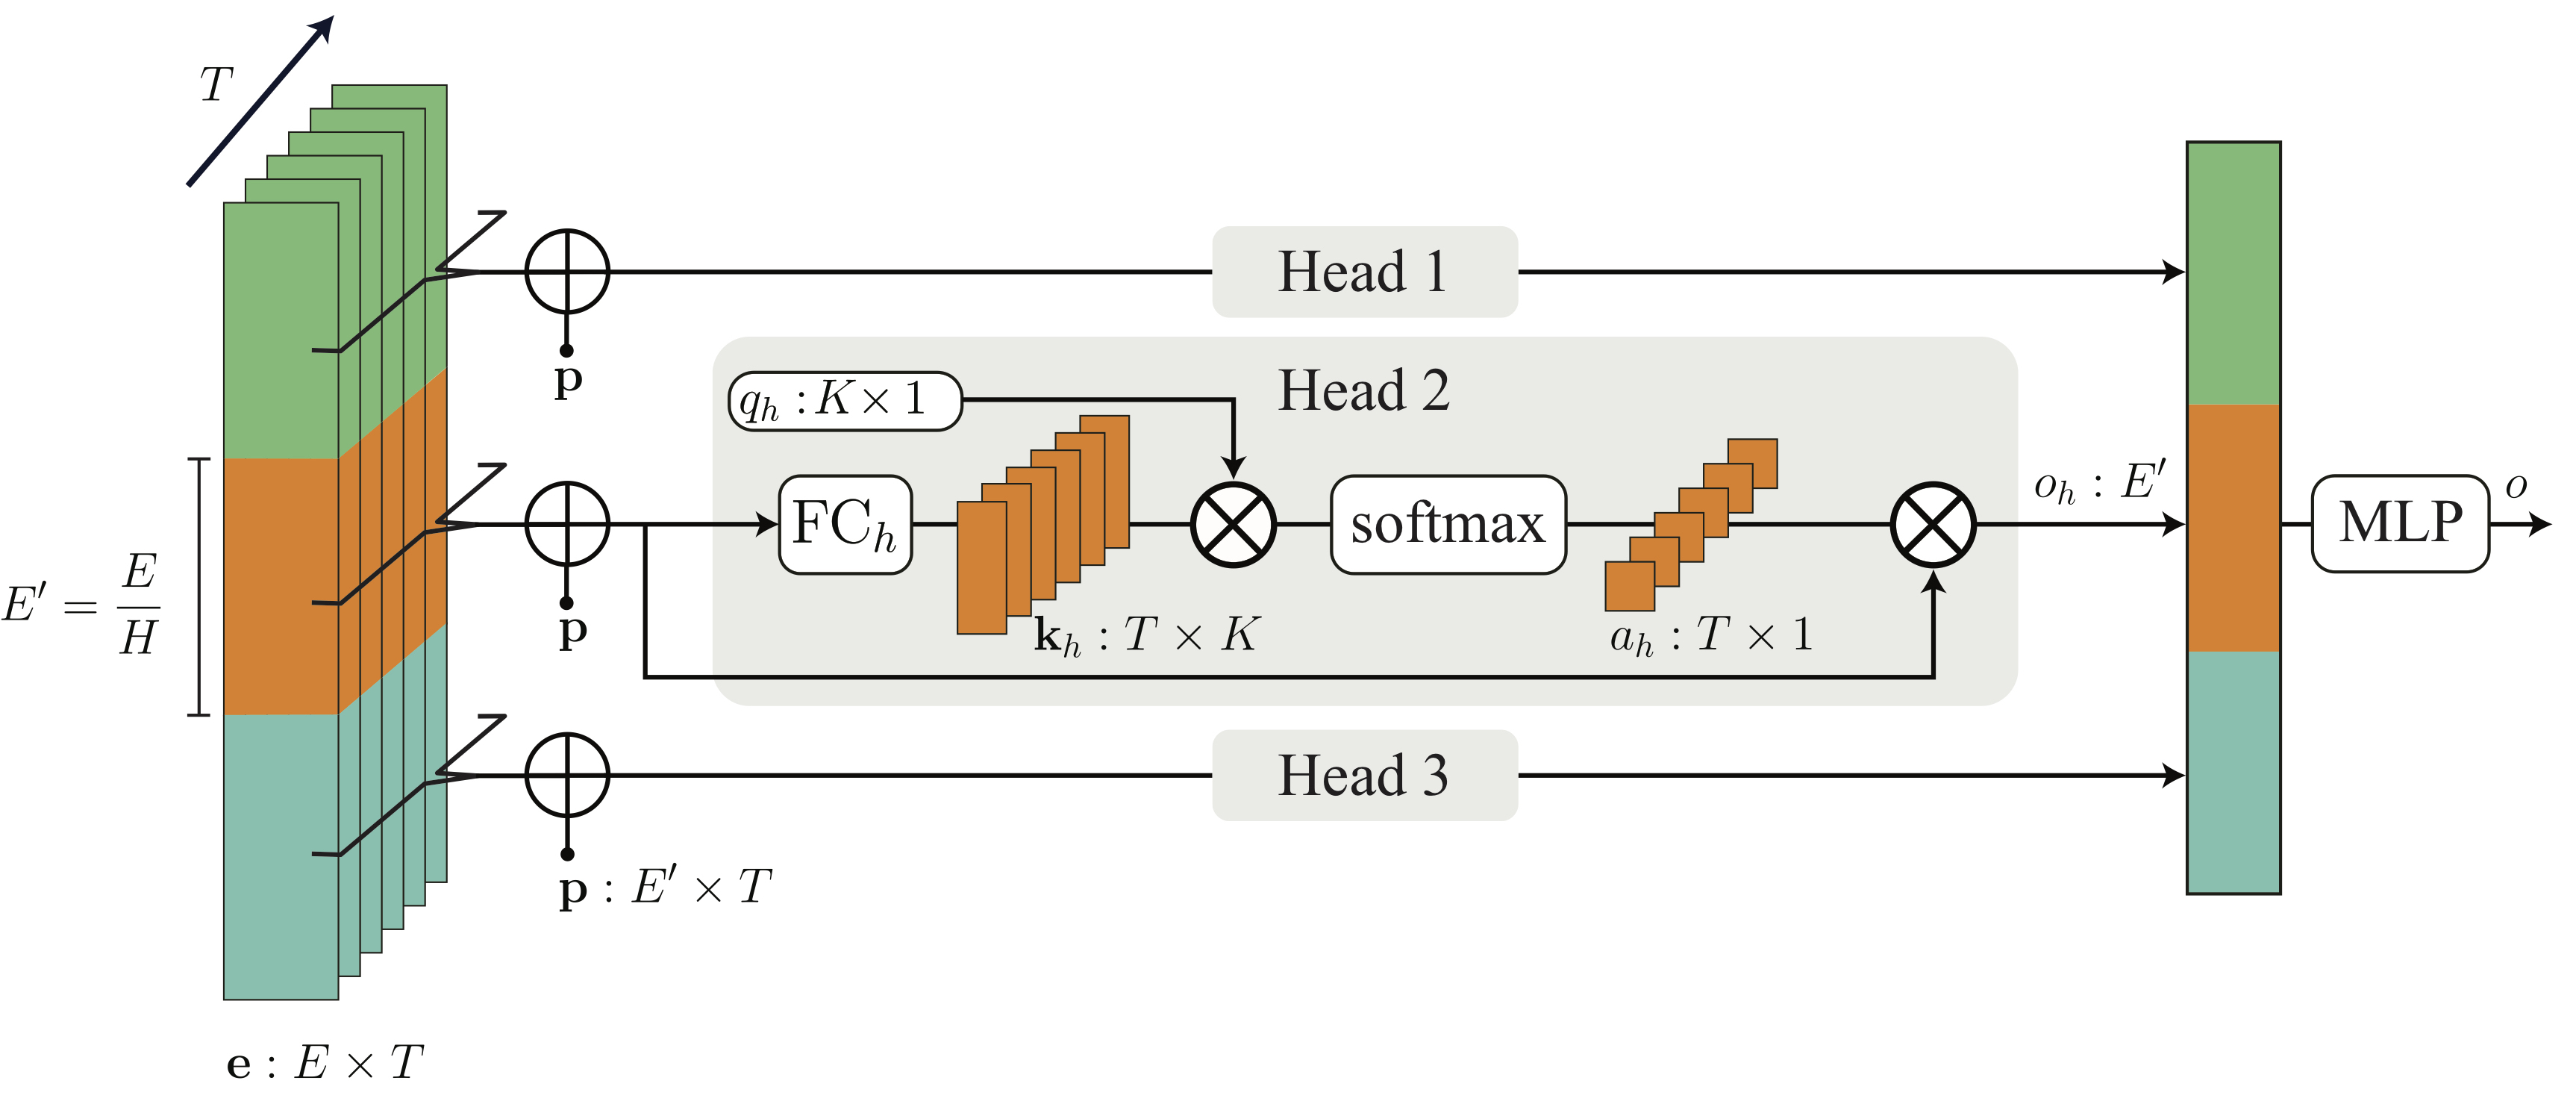
\includegraphics[width=1\textwidth]{LTAE}
  \caption{Light Temporal Attention Encoder  (L-TAE) module processing an input sequence e of $T$ vectors of
  size $E$, with $H = 3$ heads and keys of size $K$. The channels of the input embeddings
  are distributed among heads. Each head uses a learnt query $q_h$, while a linear layer
  $FC_h$ maps inputs to keys. The outputs of all heads are concatenated into a vector with
  the same size as the input embeddings, regardless of the number of heads \cite{LTAE}}
  \label{tab:LTAErchitecture}
\end{figure}

\begin{paragraph}{Channel Grouping} we propose to split the E channels of the input elements
into H groups of size E0 = E/H with H being the number of heads1
, in the
manner of Wu et al. [14]. We denote by e(t) h
the groups of input channels for the
h-th group of the t-th element of the input sequence (1).
We encode the number of days elapsed since the beginning of the sequence
into an E0 -dimensional positional vector p of characteristic scale $t$ = 1000 (2).
In order for each head to access this information, p is duplicated and added to
each channel group. Each head operates in parallel on its corresponding group
of channels, thus accelerating the costly computation of keys and queries. This
also allows for each head to specialize alongside its channel group, and avoid
redundant operations between heads.
\end{paragraph} 

\begin{paragraph}{Query-as-Parameter} 
We define the K-dimensional master query qh of each head
h as a model parameter instead of the results of a linear layer. The immediate
benefit is a further reduction of the number of parameters, while the lack of
flexibility is compensated by the larger number of available heads.
\end{paragraph} 

\begin{paragraph}{Attention Masks}
Attention Masks: As a result, only the keys are obtained with a learned linear
layer (3), while values are bypassed (v(t) = e(t)
), and the queries are model
parameters. The attention masks ah  [0, 1]T of each head h are defined as the
scaled softmax of the dot-product between the keys and the master query (4).
The outputs oh of each heads are defined as the sum in the temporal dimension
of the corresponding inputs weighted by the attention mask ah (5). Finally,
the heads outputs are concatenated into a vector of size E and processed by a
multi-layer perceptron MLP to the desired size (6). In Figure 1, we represent a
schematic representation of our network. The different steps of the L-TAE can
also be condensed by the following operations, for h = 1 · · · H and t = 1 · · · T:
\end{paragraph}

\begin{table}[ht]
  \centering
  \begin{tabular}{l p{12cm}}   
     Param & Description \\[0.2cm] 
     \hline \\[-0.2cm]  
     E & size of the embeddings ($E$), if input vectors are of a different size, a linear layer is used to project them d\_model-dimensional space \\
     H & Number of attention heads  \\
     K & Dimension of the key and query vectors  \\
     MLP & Number of neurons in the layers of MLP \\
  \end{tabular}
  \caption{Params of L-TAE model}
  \label{tab:LTAEconfig}
\end{table} 

\subsubsection{Data preparation}
%- splits\\

As described in Section \ref{sec:tempCNNDataPreparation}, we partitioned the dataset into three subsets: training (60\%), validation (20\%), and test (20\%). 
To ensure that each set had a similar class distribution and to avoid spatial autocorrelation, we took necessary precautions.

The implementation of the model was carried out using PyTorch framework. For the purpose of embedding input images, the Pixel Set Encoder (PSE) was utilized, which has previously been shown to be a suitable technique for satellite image datasets \cite{garnot2020satellite}.

While the PSE method worked well for the original dataset, we developed a new encoder called Dense Encoder (DE) that better suited the needs of our dataset.
The DE is a simple linear neural network that takes a 16-channel image as input and produces a 64-dimensional vector using a hyperbolic tangent (tanh) activation function. 
The DE was designed to be computationally efficient, allowing for faster training and inference times, while still maintaining strong performance on our specific dataset.

% - dates\\
% - pytorch implementation\\
% - PixelSetEncoder\\
% - DenseEncoder\\
% -- tanh

\subsubsection{Experimental results}

Table \ref{tab:LTAEresults} presents the performance results of the L-TAE architecture with different configurations of the following hyper-parameters: number of heads H, dimension of keys K, and number of channels E in the input sequence.
All the results were obtained through a 4-fold cross-validation scheme.
The performance metrics were measured for two different scenarios: one where missing values were imputed and one where missing values were not imputed.

\begin{table}[ht]
  \centering
  \begin{tabular}{cccclrr} 
     Params & E & H & K & MLP & No imputation & Pre imputation\\[0.2cm] 
     \hline \\[-0.2cm] 
     43k & 	128 & 	8 & 	8 & 	128 & 	$93.37 \pm 1.65$ & 	$93.08 \pm 1.16$\\ 
     68k & 	128 & 	16 & 	8 & 	128 - 128 & 	$93.43 \pm 1.37$ & 	$93.39 \pm 1.16$\\ 
     123k & 	256 & 	16 & 	8 & 	256 - 128 & 	$93.15 \pm 1.72$ & 	$93.44 \pm 1.22$\\ 
     299k & 	512 & 	32 & 	8 & 	512 - 128 & 	$\mathbf{93.65 \pm 1.30}$ & 	$93.40 \pm 1.16$\\ 
     749k & 	1024 & 	32 & 	8 & 	1024 - 256 - 128 & 	$92.91 \pm 1.90$ & 	$\mathbf{93.58 \pm 1.29}$\\ 
  \end{tabular}
  \caption{Results of the L-TAE model with different parameters}
  \label{tab:LTAEresults}
\end{table}

Overall, the results reported in Table \ref{tab:LTAEresults} demonstrate the effectiveness of the L-TAE architecture in accurately classifying the input data even with a lower number of parameters. The inclusion of missing data through imputation did not significantly impact the performance of the model, suggesting that the L-TAE architecture is robust to the presence of missing values.